\subsection{Overview}
\begin{frame}
    To answer this question we considered two modeling approaches:
    \begin{enumerate}
      \item \texttt{RAVEN} (INL) - Risk Analysis and Virtual Environment \cite{baker_optimal_2018}\cite{epiney_report_2017}
      \item \texttt{TEMOA} (NCSU) - Tools for Energy Model Optimization and Analysis \cite{decarolis_modelling_2016}\cite{decarolis_temoa_2010}\cite{hunter_modeling_2013}
    \end{enumerate}
    \vspace{0.5cm}
    Both modeling tools are open source and use publicly available version control
    software, \texttt{Git}, to track changes. \\

    The analysis in \texttt{RAVEN} requires some external modules that are not currently
    available to the public.
\end{frame}

\subsection{Methods for \texttt{RAVEN}}
\begin{frame}
  \frametitle{Workflow in RAVEN}
  \begin{figure}
    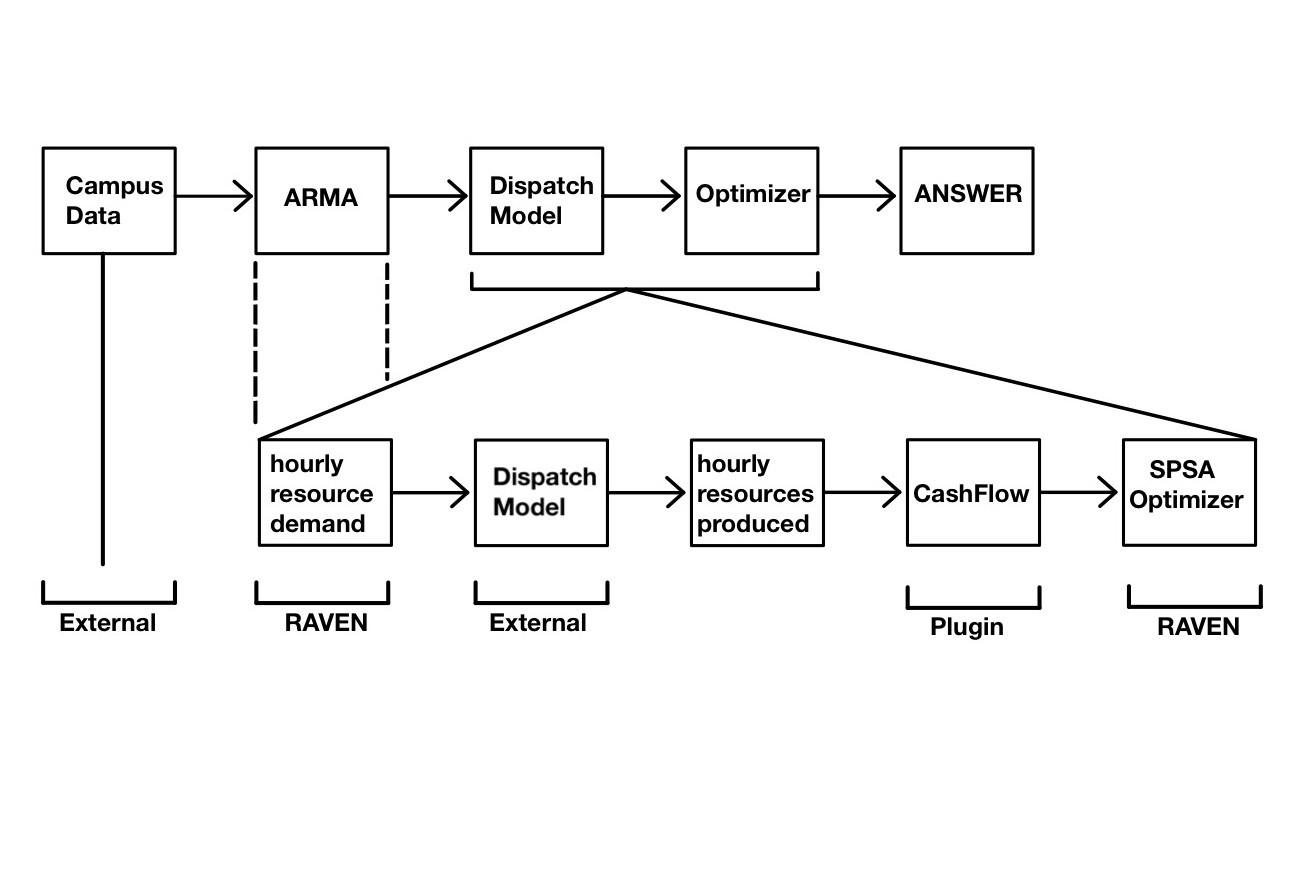
\includegraphics[width=0.8\textwidth]{raven_workflow.jpg}
    \caption{A general optimization workflow in RAVEN. Only the ARMA step was used to characterize the UIUC grid.}
    \label{fig:workflow}
  \end{figure}
\end{frame}

\subsection{Methods for \texttt{Temoa}}
\begin{frame}
  \frametitle{\texttt{Temoa} Implementation}
  \texttt{Temoa} uses linear optimization to search decision space \cite{hunter_modeling_2013}.
  \begin{enumerate}
    \item Objective Function (minimizes system cost)
    \item Constraints
    \begin{enumerate}
      \item Demand must be satisfied at each time step (always).
      \item Carbon limits must be satisfied at each time step (optionally).
    \end{enumerate}
    \item Variables
    \begin{enumerate}
      \item Cost
      \item Generation
      \item Capacity
    \end{enumerate}
  \end{enumerate}
\end{frame}
